cd ~/%!TEX root = ../dokumentation.tex


\chapter{Implementation}\label{cha:Implementation}

\section{Lexer}\label{sec:ImplementationLexer}

As mentioned in chapter \ref{sec:ConceptLexer} the implementation of the lexer consists of the definition of tokens in form of regular expression. The following paragraph presents defined tokens and their regular expressions.

\subsubsection{Ignored symbols}
It is possible to declare symbols that should be ignored. However, if a symbol is declared as ignored but is specially mentioned in another token, then if the sequence
of characters represent that token, the ignored symbol is not ignored. In this project, tabs and white spaces are ignored as they do not have any special meaning other than providing clarity.
Also, newlines are generally ignored because as can be seen in listing \ref{lst:Lexer_example_multiline} there are rules that cover multiple lines.

\begin{lstlisting}[basicstyle=\scriptsize	,caption= Multi line production rule,label= lst:Lexer_example_multiline]
<annotated_formula>    ::= <thf_annotated> | <tff_annotated> | <tcf_annotated> |
                           <fof_annotated> | <cnf_annotated> | <tpi_annotated>
\end{lstlisting}

Apart from the ignored symbols, there are 13 defined tokens:

\subsubsection{Expressions}

Expressions can either be of the type grammar, token, strict or macro. It is defined as a nonterminal symbol followed by the production symbol itself (::=,:==,:::,...). The nonterminal symbol and the production are merged to a single token and are not identified as two tokens to avoid ambiguity while parsing. If not it would be difficult for the parer to determine whether the nonterminal symbol that describes the rule is the start of a new rule or does still belong to the previous rule because as mentioned rules can cover multiple lines.

\textit{Regular expression of grammar expression:}  $'<\backslash w+>[\backslash s]*::='$

$\backslash w+$ matches any alphanumeric and underscore character that can occur more than one time.
$[\backslash s]*$ matches an arbitrary amount of white spaces.

\subsubsection{Nonterminal symbol}

A nonterminal symbol starts with \dq <\dq and ends with \dq >\dq. In between there is any arbitrary sequence of numbers, underscores and small or capital letters.

\subsubsection{Terminal symbol}

\subsubsection{Comment}

A comment is identified by the lexer as a start of a new line followed by a percentage sign followed by an arbitrary character and ends with a newline. Because the percentage sign is also part of the terminal symbols, it is necessary to check whether the percentage sign is in a newline because the terminal symbol is not because the percentage symbol when used as terminal symbol is embedded in square brackets.    

\subsubsection{Meta-Symbols}

Meta-Symbols include open and close parentheses \dq( )\dq, open and close square brackets \dq[ ]\dq, asterisks \dq *\dq and vertical bars \dq |\dq.

They are recognized by the symbol itself and have a greater meaning for the parser as they impact the to be build data structures. 

\subsubsection{Ambiguity}

The following example could either be matched as one comment token or as comment, grammar expression, non terminal symbol, terminal symbol, non terminal symbol.
This ambiguity is solved because by convention the lexer matches the longest possible token, the sequence of characters is matched as one comment.
\begin{lstlisting}[basicstyle=\scriptsize	,caption= Commented out production rule,label= lst:Lexer_example]
%----   <formula_role> ::= <user_role>-<source>
\end{lstlisting}
\section{Parser}\label{sec:ImplementationParser}

The parser is taking the tokens from the lexer and matches them to defined production rules.




comment block reimplement equal operator

\subsection{Data types}\label{sec:ImplementationDataTypes}
Figure \ref{fig:ImplementationUMLExpressions} contains the UML modelling of the data types described in section \ref{sec:ConceptParserDataStructure}.
\begin{figure}[H]
\centering
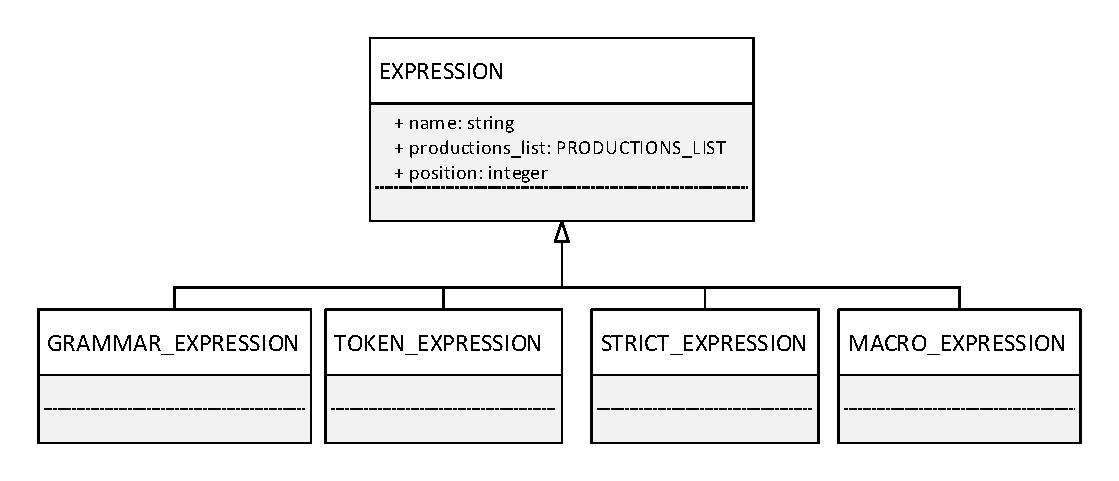
\includegraphics[width=1\textwidth]{images/uml_data_types_expressions.pdf}
\caption{UML diagram for expressions}
\label{fig:ImplementationUMLExpressions}
\end{figure}


\begin{figure}[H]
\centering
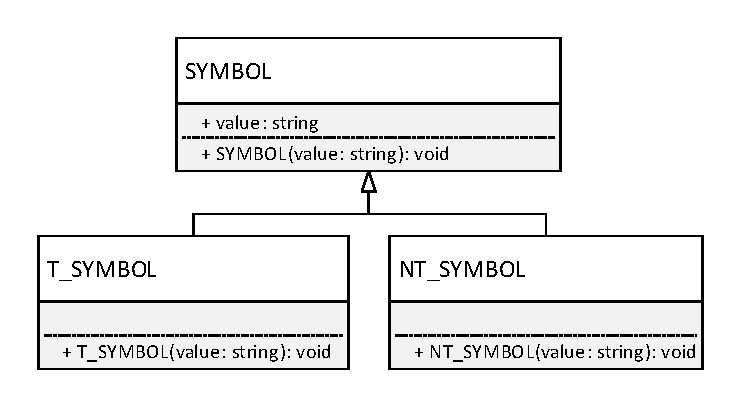
\includegraphics[width=.7\textwidth]{images/Implementation_parser_symbol_uml.pdf}
\caption{Symbols UML diagram}
\label{fig:ImplementationUMLSymbols}
\end{figure}


\subsection{Defined grammar}\label{sec:ImplementationGrammar}

- Input of parser is formal grammar \\

The grammar is formally specified $G = (N,\sum,P,S)$.

$N$ is the set of nonterminal symbols. The set includes grammar list, comment block, grammar expression, token expression, strict expression, macro expression, productions list, production, xor productions list, t symbol production and production element.

$\sum$ is the set of terminal symbols. Terminal symbols of the specified grammar are the tokens generated by the lexer (see \ref{sec:ConceptLexer}).

$P$ is the set of production rules that are presented in the following. 

A grammar list implies a comment block, the four expressions or a grammar list followed by the expressions.

\begin{align*}
	grammar\;list\; \rightarrow\; &comment\;block
	     		\mid grammar\;expression  \\
			   &\mid token\;expression
                \mid strict\;expression\\
               &\mid macro\;expression \\
               &\mid grammar\;list\;\;\;grammar\;expression\\
               &\mid grammar\;list\;\;\;strict\;expression \\
               &\mid grammar\;list\;\;\;macro\;expression \\
               &\mid grammar\;list\;\;\;comment\;block               
\end{align*}

A comment block is either a comment or a comment block with a comment.

\begin{align*}
    comment\;block\; \rightarrow\; &\textbf{comment}
                \mid comment\;block\;\;\textbf{comment}
\end{align*}

The four expressions are the expression token followed by their productions list. Grammar expression has a special case without a productions list because the production rule $ <null> ::= $ has nothing on the right side. 

\begin{align*}
	grammar\;expression\; \rightarrow\; &\textbf{l grammar expression}\;\;productions\;list \\ 
               &\mid \textbf{l grammar expression} 
\end{align*}
\begin{align*}        
	token\;expression\; \rightarrow\; &\textbf{l token expression} \;\;productions\;list \\ \\
	strict\;expression\; \rightarrow\; &\textbf{l strict expression} \;\;productions\;list \\ \\
	macro\;expression\; \rightarrow\; &\textbf{l macro expression} \;\;productions\;list 
\end{align*}

Productions list and xor productions list imply either a production or a productions list alternative symbol production.
\begin{align*}
        productions\;list\; \rightarrow\; &production \\
               &\mid productions\;list\;\;\textbf{alternative symbol} \;production \\ \\                  
        xor\;productions\;list\; \rightarrow\; &production \\
               &\mid xor\;productions\;list\;\;\textbf{alternative symbol}\;production
\end{align*}
T symbol production is either a t symbol or a t symbol/repetition symbol/ alternative symbol embedded in square brackets.

\begin{align*}
	t\;symbol\;production\; \rightarrow\; & \textbf{open square bracket \; t symbol} \\ &\textbf{close square bracket}\\
               &\mid \textbf{open square bracket \; repetition symbol} \\ &\textbf{close square bracket}\\
               &\mid \textbf{open square bracket \; alternative symbol } \\ &\textbf{close square bracket}\\
               &\mid \textbf{t symbol} 
\end{align*}

Production element can be replaced by a nt symbol or by a nt symbol in square brackets or nt symbol repetition. In the case of repetition or square brackets the production element is categorized as optional when in square brackets or as repetition when followed by the repetition symbol. The same applies to t symbol production. A production element can also only be square brackets only.

 

\begin{align*}
	production\;element\; \rightarrow\; & \textbf{open square bracket \; nt symbol} \\ 
			   &\textbf{close square bracket}\\
               &\mid \textbf{nt symbol \; repetition symbol} \\
               &\mid t\;symbol\;production\;\; \textbf{repetition symbol} \\
               &\mid \textbf{open square bracket \; close square bracket} \\
               &\mid \textbf{nt symbol} \\
               &\mid t\; symbol\; production 
\end{align*}




\begin{align*}
	production\; \rightarrow\; &production\; element
                \mid production\;\; production\; element \\
               &\mid \textbf{open parenthesis}\;\; xor\; \;productions\; list\;\; \\
               &\textbf{close parenthesis} \\
               &\mid \textbf{open parenthesis}\;\; production\;\; \textbf{close parenthesis} \\
               &\mid production \;\;\textbf{open parenthesis}\;\; production \\
               &\textbf{close parenthesis} \\
               &\mid production\;\; \textbf{open parenthesis} \;\;xor \;productions\; list\\
               &\textbf{close parenthesis} \\
               &\mid \textbf{open parenthesis} \;\;production \;\;\textbf{close parenthesis} \\
               &production \\
               &\mid \textbf{open parenthesis}\;\; xor\; productions\; list\\ 
               &\textbf{close parenthesis}\;\; production \\
               &\mid \textbf{open parenthesis}\;\; production\;\; \textbf{close parenthesis} \\
               &\textbf{repetition symbol}\\
               &\mid production\;\; \textbf{open parenthesis} \;\;production \\
               &\textbf{close parenthesis \; repetition symbol}
\end{align*}


- $S$: grammar list, start symbol is not mentioned, per convention by \ac{PLY} first rule found (top level rule)

Listing \ref{lst:Parser_example_productionelement} shows the production rule of the nonterminal $<tfx tuple>$ as well as the tokens that have been generated by the lexer.

\begin{lstlisting}[basicstyle=\scriptsize	,caption= Production element,label= lst:Parser_example_productionelement]
<tfx_tuple>            ::= [] | [<tff_arguments>]
is made of tokens:
l grammar expression open square bracket close square bracket alternative symbol open square bracket nt symbol close square bracket
\end{lstlisting}

The resulting parse tree can be seen in figure \ref{fig:ImplementationParsing}. 

\begin{figure}[H]
\begin{tikzpicture}[
  ->,>=stealth',
  level/.style={level distance=1.5cm,sibling distance=4cm},
  level 2/.style={sibling distance=6cm},
  level 3/.style={sibling distance=5cm},
  level 5/.style={level distance=2cm, sibling distance=4cm},
  level 6/.style={level distance=2cm, sibling distance=4cm}
]
\node {grammar list}
    child{ node  {grammar expression} 
    		child{ node {\textbf{l grammar expression}}}
            child{ node {productions list} 
                child{ node  {productions list}
                	child {node {production}
                		child {node {productions element}
                			child{node {\textbf{\shortstack{open square bracket \\ close square bracket}}}}}}} 
                child{ node  {\textbf{alternative symbol}}}
                child{ node  {production}
                	child {node {productions element}
                		child{node {\textbf{\shortstack{open square bracket \\ nt symbol \\ close square bracket }}}}}}
                				}}
   
; 
\end{tikzpicture}
\caption{Parsing example}
\label{fig:ImplementationParsing}
\end{figure}
                
                
                
\section{Graph generation}\label{sec:ImplementationGraphGeneration}

To generate the graph of a given grammar three algorithms are needed that will be explained in the following. 

The algorithm $buildGraphRek$ calls the function $searchProductionsListForNT$ that appends children of a node to the nodes list of children. The algorithm is first called with the start symbol. 
After the children of a node have been appended to the node, every child calls the algorithm resulting in appending their own children to their children's list. 

\begin{algorithm}[H]
\caption{Graph Generation Algorithm: buildGraphRek}
\begin{algorithmic}[1] 
\Require node
%\ENSURE $y = x^n$
\State searchProductionsListForNT(node, node.productionsList)
\If {node has children}
	\ForAll {children}
		\State buildGraphRek(child)
	\EndFor
\EndIf
\end{algorithmic}
\end{algorithm}

The right side of a production rule is stored in a productions list. For identifying the nonterminal or terminal symbols in the productions lists, a loop iterates through all elements of the productions list. Each element is a production and calls the function $searchProductionForNT$. This function identifies the children of the given element who are then appended to the node.

\begin{algorithm}[H]
\caption{Algorithm for extracting productions from productions list: searchProductionsListForNT}
\begin{algorithmic}[1] 
\Require node, productionsList
\ForAll {elements in productionsList}
	\State children = new empty list
	\State searchProductionForNT(node, element in productionsList, children)
	\State append children to node
\EndFor
\end{algorithmic}
\end{algorithm}

The goal is to identify the nonterminal symbols. Therefore it is checked if the production is a nested production and if so, the same function is called again. If the production is a XOR production list the function $searchProductionsListForNT$ is called to break down the productions list. If the production element is a nonterminal symbol the element is searched in the node dictionary to get the node where the element is on the left side. This element is then appended to a list of children. It is possible that an element appears multiple times on the left side if it is presented by multiple expressions. In this case each element is appended to the list of children.

\begin{algorithm}[H]
\caption{Algorithm for appending children to node: searchProductionForNT}
\begin{algorithmic}[1] 
\Require node, productionsElement, children
\ForAll {elements in productionsElementList}
	\If {element is  a production}
		\State {searchProductionForNT(node, element, children)}
	\ElsIf {element is a XOR productions list}
		\State {searchProductionsListForNT}
	\ElsIf {element is a nonterminal symbol}
		\State find element(s) in node dictionary
		\State append element(s) to children
	\EndIf
\EndFor
\end{algorithmic}
\end{algorithm}

\section{Extraction of a sub-syntax}\label{sec:ImplementationExtractReducedGrammar}
The following sections describe the algorithms for the extraction of a sub-syntax based on the concept outlined in section \ref{sec:ConceptExtractReducedGrammar}

\subsection{Removal of blocked productions}
Algorithm \ref{alg:remove_blocked_productions} takes the text of the control file as an input argument (control file format description can be found in section \ref{sec:ConceptControlFile}) and removes the productions, that should be blocked, from the nodes.  
The control file string is split into a list of the lines (line 1).
The first line of the control file string, which describes the start symbol, is deleted from the list (line 2) because this information is not needed at this step.\\
Then the following lines are iterated:\\
For each line the content is split by the comma symbol, which produces a list of strings.
The first element of that list is the nonterminal symbol name of the symbol of which productions should be disabled.
The second element is the corresponding rule type symbol.
The nonterminal symbol name and the rule type, that is determined from the rules symbol (line 7), are stored in separate variables.
Then these elements are removed from the list and the remaining elements are converted to integer.
They are the indexes of the productions that should be removed.
The elements are ordered in a descending order (line 10).
Ordering the indexes in that order has the advantage that, when the list of indexes is iterated to delete productions, the indexes of other productions that should be deleted are not changed by the deletion of productions before. ?todo verständlich?
To delete the productions from the specified node, the node object has to be obtained.
This is done by addressing the node in the \textit{nodes\textunderscore dictionary} with its key consisting of the nonterminal symbol name and the rule type.
From the node, in a loop, the elements of the \textit{productions\textunderscore list} and the \textit{children} list corresponding to the indexes in the control file are deleted.

\begin{algorithm}[H]
\caption{Removing blocked productions}
\begin{algorithmic}[1] 
\Require control\textunderscore string
\State lines = control\textunderscore string.splitlines()
\State delete lines[0]
\ForAll {line in lines}
	\State data = line.splitBy(",")
	\State nonterminal\textunderscore name = data[0]
	\State rule\textunderscore symbol = data[1]
	\State rule\textunderscore type = determineRuleType(rule\textunderscore symbol)
	\State delete data[0:2]
	\State data = parseInteger(data)
	\State data.sortReverse()
	\State node = this.nodes\textunderscore dictionary.get(Node\textunderscore Key(nonterminal\textunderscore name, rule\textunderscore type))
	\ForAll {index in data}
		\State delete node.productions\textunderscore list.list[index]
		\State delete node.children[index]
	\EndFor
\EndFor
\end{algorithmic}
\label{alg:remove_blocked_productions}
\end{algorithm}

\subsection{Determination of the remaining terminating symbols}
After the desired productions have been deleted from the grammar graph, the next step is to remove the nonterminating symbols from the grammar graph. Algorithm \ref{alg:remove_non_terminating_symbols} shows the procedure of how to remove nonterminating symbols.
First it has to be determined which symbols are terminating and which are nonterminating.

-one way: starting from terminal symbol, find nonterminal symbol that derives terminal symbol, then find nonterminal symbol that only produces terminating symbols
-graph data structure can only be traversed top down not bottom up.
-therefore start at start node, traverse graph, and find terminating symbols
-initialise visited set
-store known terminating symbols

A set of terminating nodes and a temporary set of terminating nodes are initialized.
In the while loop the recursive algorithm find\textunderscore non\textunderscore terminating\textunderscore symbols(start\textunderscore node, temp\textunderscore terminating, visited) finds terminating nodes with the start\textunderscore node, and an initialized set of known terminating symbols and a set of already visited nodes.
This algorithm is called with the ?updated? set of terminating symbols until the set does not differ from the run before.
When that is the case all terminating nodes have been found.\\
After all terminating nodes have been found, the productions that contain nonterminating symbols are deleted from the nodes and after that nodes representing nonterminating symbols are removed.

\begin{algorithm}[H]
\caption{Removing non terminating symbols}
\begin{algorithmic}[1] 
\Require start\textunderscore node
\State terminating = new set()
\State temp\textunderscore terminating = new set()
\While {True}
	\State visited = new set()
	\State this.find\textunderscore non\textunderscore terminating\textunderscore symbols(start\textunderscore node, temp\textunderscore terminating, visited)
	\If {terminating == temp\textunderscore terminating}
		\State break
	\Else
		\State terminating = temp\textunderscore terminating
	\EndIf
\EndWhile
\State visited = new set() 
\State delete\textunderscore non\textunderscore terminating\textunderscore productions(start\textunderscore node, terminating, visited)
\State delete\textunderscore non\textunderscore terminating\textunderscore nodes(terminating)
\end{algorithmic}
\label{alg:remove_non_terminating_symbols}
\end{algorithm}


Algorithm \ref{alg:find_non_terminating_symbols} 
determines whether a node can be identified as terminating by recursive checking

The input are a set of already known terminating nodes and nodes that already have been visited.
recursive
If the node has been not been visited before it is added to the visited set and...
If it has been visited before, the method ?todo? ends to prevent infinite loops
for each children list in node.children
-if len list 0, only terminal symbols in productions, that means node certainly terminating
-else: check if all childs in children list are terminating, by recursive call
-if after that node not in terminating then not known that it is terminating
-if terminating add to known terminating symbols

\begin{algorithm}[H]
\caption{Find non terminating symbols}
\begin{algorithmic}[1] 
\Require node, terminating\textunderscore set, visited\textunderscore set
\State node\textunderscore key = Node\textunderscore Key(node.value, node.rule\textunderscore type)
\If {node\textunderscore key not in visited\textunderscore set}
	\State visited\textunderscore set.add(node\textunderscore key)
	\ForAll {children\textunderscore list in node.children}
		\If{len(children\textunderscore list) == 0}
			\State terminating\textunderscore set.add(node\textunderscore key)
		\Else
			\State terminating\textunderscore flag = True
			\ForAll {child in children\textunderscore list}
				\State find\textunderscore non\textunderscore terminating\textunderscore symbols(child, terminating\textunderscore set, visited\textunderscore set)		
				\If {not value\textunderscore in\textunderscore terminating(child.value, terminating\textunderscore set)}
					\State terminating\textunderscore set = False
				\EndIf
			\EndFor
			\If {terminating\textunderscore flag}
				\State terminating\textunderscore set.add(node\textunderscore key)
			\EndIf
		\EndIf
	\EndFor
\EndIf
\end{algorithmic}
\label{alg:find_non_terminating_symbols}
\end{algorithm}

-recursive
-if not visited
-add to visited
-index to end
For each child the algorithm is called recursively. If the child node does not correspond to a terminating symbol, set nonterminating flag to ture
If the nontermiating flag is true, delete production -> delete children entry and productions list entry.
-value in terminating checks if any ?rule type? is terminating

-call for each child in children list
-if child not in terminating, set not terminating flag
-if not terminating, delete corresponding children list and prouctions list


-todo check children list, ist was wenn symbol mehrere nodes hat?

Algorithm \ref{alg:delete_non_terminating_productions} 
\begin{algorithm}[H]
\caption{Delete non terminating productions}
\begin{algorithmic}[1] 
\Require node, terminating\textunderscore set, visited\textunderscore set
\State node\textunderscore key = Node\textunderscore Key(node.value, node.rule\textunderscore type)
\If{node\textunderscore key not in visited\textunderscore set}
	\State visited\textunderscore set.add(node\textunderscore key)
	\State index = len(node.children) - 1
	\ForAll {children\textunderscore list in reversed(node.children)}
		\State not\textunderscore terminating = False
		\ForAll {child in children\textunderscore list}
			\State delete\textunderscore non\textunderscore terminating\textunderscore productions(child, terminating\textunderscore set, visited\textunderscore set)
			\If{not value\textunderscore in\textunderscore terminating(child.value, terminating\textunderscore set)}
				\State not\textunderscore terminating = true
			\EndIf
		\EndFor
		\If{not\textunderscore terminating}
			\State delete node.children[index]
			\State delete node.productions\textunderscore list.list[index]
		\EndIf
		\State index = index - 1
\EndFor
\EndIf
\end{algorithmic}
\label{alg:delete_non_terminating_productions}
\end{algorithm}


Algorithm \ref{alg:delete_non_terminating_nodes} removes the nonterminating nodes from the \textit{nodes\textunderscore dictionary}. It takes a set of \textit{Node\textunderscore Keys}s as input, that specifies all terminating nodes as input.
To remove the nonterminating nodes, in a for-loop, all terminating nodes that are addressed by the \textit{Node\textunderscore Key}s are stored in a temporary dictionary. This dictionary replaces the original \textit{nodes\textunderscore dictionary} of the \textit{TPTPGraphBuilder}.
\begin{algorithm}[H]
\caption{Delete non terminating nodes}
\begin{algorithmic}[1] 
\Require terminating\textunderscore set
\State temporary\textunderscore dictionary = \{\}
\ForAll{node\textunderscore key in terminating\textunderscore set}
	\State value = this.nodes\textunderscore dictionary.get(node\textunderscore key, None)
	\State temporary\textunderscore dictionary.update({node\textunderscore key: value})
\EndFor
\State this.nodes\textunderscore dictionary = temporary\textunderscore dictionary
\end{algorithmic}
\label{alg:delete_non_terminating_nodes}
\end{algorithm}



\subsection{Determination of the remaining reachable ?productions?}
As mentioned in section \ref{sec:ConceptRemovingBlockedProductions} todo check reference the determination of the remaining reachable is done by creating a new grammar graph, with the desired start symbol from the control file. The nodes dictionary is also reduced to contain only the reachable nodes. 

\section{Output generation}\label{sec:ImplementationOutputGeneration}
\subsection{Create output from grammar graph}\label{sec:ImplementationOutputGrammarGraph}

\subsection{Traverse graph to create string representations of objects}\label{sec:ImpolementationOutputGrammarGraphTraverse}

\subsection{Create string representations of objects}\label{sec:ImplementationOutputGrammarGraphStringRepresentations}

- python has string class \url{https://docs.python.org/3/library/stdtypes.html#str}
- returns string version of the passed object
- it returns object.\textunderscore \textunderscore str \textunderscore \textunderscore () when object has the method
- following classes implement str method:

COMMENT\textunderscore  BLOCK
-lines from lines list with newline

PRODUCTION\textunderscore ELEMENT

PRODUCTION
-order

NTNODE

\subsection{Maintain original order}\label{sec:ImplementationOutputGrammarGraphMaintainOrder}
- use tuple of position and node string


\subsection{Automated parser generator compatibility}\label{sec:ImplementationAutomatedParserGenerator}
-append option

\section{Input/Output}\label{sec:ImplementationInOut}

\section{GUI}\label{sec:ImplementationGUI}
The GUI consists of the class View that can be seen in Figure \ref{fig:ImplementationViewClassDiagram}. The class has the attributes $treeView$ which is an instance of the PyQt QTreeWidget, $graphBuilder$ which is an instance of the TPTPGraphBuilder and the boolean value $commentStatus$. The class functions are described in the following.

\begin{figure}[H]
\centering
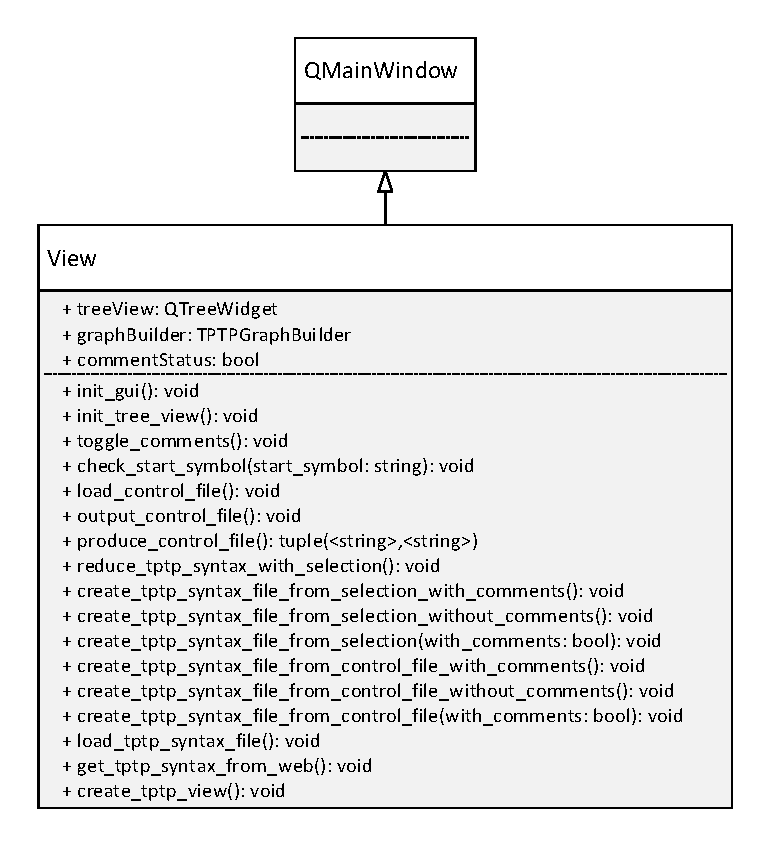
\includegraphics[width=0.8\textwidth]{images/Implementation_view_class_diagramm.pdf}
\caption{View UML class diagram}
\label{fig:ImplementationViewClassDiagram}
\end{figure}

\subsubsection{Init GUI}\label{sec:ImplementationGUIInit}

The function $init\textunderscore gui$ sets up the menu bar in the main application window. The menu bar consists of the sub-menus "Import syntax", "Save syntax", "Reduce", "Control file" and "View". To each sub-menu menu actions that have been described in chapter \ref{sec:ConceptGUI} are added and implemented using QActions. The following listing \ref{lst:ImplementationInitGUI} shows the Python code for adding a menu bar and menu actions for example for the "Import syntax" menu bar.

\begin{lstlisting}[language=Python, basicstyle=\scriptsize	,caption= Implementation of menu bar,label= lst:ImplementationInitGUI]
import_menu = menubar.addMenu("Import syntax")
import_menu.addAction(import_tptp_file_action)
import_menu.addAction(import_tptp_file_from_web_action)
\end{lstlisting}

Besides a name, a short cut for executing the menu action is defined. Also triggers have been defined that triggers functions once menu button is pressed. Listing \ref{lst:ImplementationInitGUI2} shows how a short cut and a trigger have been defined for the action $Import TPTP syntax file$.

\begin{lstlisting}[language=Python, basicstyle=\scriptsize	,caption= Implementation of menu actions,label= lst:ImplementationInitGUI2]
import_tptp_file_action = QAction('&Import TPTP syntax file', self)
import_tptp_file_action.setShortcut('Ctrl+O')
import_tptp_file_action.triggered.connect(self.load_tptp_syntax_file)
\end{lstlisting}


\subsubsection{Init TreeView}\label{sec:ImplementationGUIInitTreeView}
A new tree view is defined using QTreeWidget with the header labels "Nonterminal", "Production Type" and "Production".

All node names of the nodes dictionary of the GraphBuilder instance are extracted and sorted based on their position in the original \ac{TPTP} syntax file. For every node a new QTreeWidgetItem is generated with the node.value and rule type. Also a new checkbox is defined whose initial value is unchecked. The background to set to grey.
For every production in the nodes production list, also a new QTreeWidgetItem and Checkbox are created, However, the default value is set un unchecked. The generated item is then added as a child to the previous? item. A comment block is set as toplevelitem and flags of the item are set accordingly.
	
\subsubsection{Check start symbol}\label{sec:ImplementationGUIStartsymbol}

This function checks the checkbox of the defined start symbol. The QTreeView method $findItem(string\; itemName)$ is used that returns all items that match the item name. 
The found items are than checked.

\subsection{Display rules}\label{sec:ImplementationGUIDisplayRules}

\subsubsection{Toggle comments}\label{sec:ImplementationGUIToggleComments}

Algorithm \ref{alg:toggleComments} shows the algorithm used for toggling comments.
The View class attribute $commentStatus$ indicates whether comments are displayed (true) or not (false). For toggling comments, a new status is set that is the opposite of commentStatus. While looping through every item in $treeView$, comment items can be found by checking whether the item is checkable because by default a comment is not checkable by the user. A QTreeWidgetItem has flags including a flag "ItemIsUserCheckable" that is used for determining whether the item is checkable. The QTreeWidgetItem function $setHidden(bool\;hide)$ is applied on every comment with the value of the new status. CommentStatus is set to the new status. 

-flag(), bitweises AND 

\begin{algorithm}[H]
\caption{GUI Algorithm: toggle\textunderscore comments}
\label{alg:toggleComments}
\begin{algorithmic}[1] 
\State newStatus = not commentStatus
\ForAll {items in treeView}
	\If {item is not checkable}
		\State item.setHidden(newStatus)
	\EndIf
\EndFor
\State commentStatus = newStatus
\end{algorithmic}
\end{algorithm}


\subsection{Import control file}\label{sec:ImplementationGUIImportControlFile}
- open control file via QFileDialog \\
- uncheck all left symbols, check all right symbols, separate via has item parents \\
- read first line in control file, set start symbol accordingly  \\
- for each following line, read nt name and ruletype and search item and uncheck it

\subsubsection{Import \ac{TPTP} syntax from the internet}\label{sec:ImplementationGUIImportInternet}

The \ac{TPTP} syntax file is extracted from the \ac{TPTP} website using the Input method $import\textunderscore tptp\textunderscore syntax\textunderscore from\textunderscore web$ (see chapter REF). This method returns a textfile. The application opens a dialog window where the user has to specify a desired start symbol. With the textfile and the start symbol, the method $create\textunderscore tptp\textunderscore view$ is called.

\section{Command-line interface}\label{sec:ImplementationCommandLineInterface}
With the argparse module a command-line parser object can be created and parameters can be added to that object.
In the first line of listing \ref{lst:ImplementationArgparseParserConfiguration} the command-line parser object is created with a description.
Lines two to four contain the specification of the accepted arguments.
In addition to the name and short form of the name, the type, a help message, and whether the parameter is optional or not can be specified.
Default values for arguments can also be specified.
If no default value is specified and if the argument is not passed it will have the value \textit{None}.
Argparse automatically checks the given conditions, for example if a required argument is not given and displays an error message if that is the case.

todo listing describe last argument
\begin{lstlisting}[language=Python, basicstyle=\scriptsize	,caption= Argparse command-line parser configuration,label= lst:ImplementationArgparseParserConfiguration]
self.argument_parser = argparse.ArgumentParser(description='Extract sub-syntax using TPTP syntax file and a control file')
self.argument_parser.add_argument('-g', '--grammar', metavar='', type=str, required=True, help='path of the TPTP syntax file')
self.argument_parser.add_argument('-c', '--control', metavar='', type=str, required=True, help='path of the control file')
self.argument_parser.add_argument('-o', '--output', metavar='', type=str, required=False, help='optional output file name (default output.txt)', default= "output.txt")
self.argument_parser.add_argument('-ec', action='store_true', help="flag - include external comment syntax")
\end{lstlisting}

Argparse will also automatically create the help output by using the descriptions provided when configuring the argument parser.


-options for path to grammar and control file
-option for output path

-todo describe seperation of gui and why
